\documentclass[conference]{IEEEtran}

% \usepackage{cite}
\usepackage{amsmath,amssymb,amsfonts}
\usepackage{verbatim} % um viele zeilen auszukommentieren
\usepackage{algorithmic}
\usepackage{listings}
\usepackage{siunitx}
\lstset{
	language=Python,
	basicstyle=\ttfamily\small,
	aboveskip={1.0\baselineskip},
	belowskip={1.0\baselineskip},
	columns=fixed,
	extendedchars=true,
	breaklines=true,
	tabsize=4,
	frame=lines,
	showtabs=false,
	showspaces=false,
	showstringspaces=false,
	keywordstyle=\color[rgb]{0.627,0.126,0.941},
	commentstyle=\color[rgb]{0.133,0.545,0.133},
	stringstyle=\color[rgb]{01,0,0},
	numbers=left,
	numberstyle=\small,
	stepnumber=1,
	numbersep=10pt,
	captionpos=t,
	escapeinside={\%*}{*)}
}

\usepackage{hyperref}
\hypersetup{colorlinks=true, pdfstartview=FitV, linkcolor=blue, citecolor=black, plainpages=false, pdfpagelabels=true, urlcolor=blue}
\usepackage[all]{hypcap}

\usepackage{graphicx}

\usepackage[ngerman]{babel}
\usepackage[utf8]{inputenc}
\usepackage[T1]{fontenc}
\usepackage[backend=biber,defernumbers=false]{biblatex}

% Einbinden der .bib-Datei
\bibliography{Literatur}  
%-----------------------------------
\usepackage{textcomp}
\usepackage{xcolor}
\usepackage{dirtytalk} % nein, nicht was du denkst.  Packet hilft  gegen verschluckte gänsefüschen
\def\BibTeX{{\rm B\kern-.05em{\sc i\kern-.025em b}\kern-.08em T
		\kern-.1667em\lower.7ex\hbox{E}\kern-.125emX}}
\usepackage{minted}
\setminted{breaklines,breakanywhere}

% für Vektorgraphen
\usepackage{color}
\usepackage{transparent}
\graphicspath{{img/}}

% Filter
\defbibfilter{wissenschaftlich}{%
	not type=online and not type=thesis
}
\defbibfilter{nichtWissenschaftlich}{%
	type=online or type=thesis
}

\begin{document}
		
	\title{rosBerry - ein autonomer Roboter auf Basis von ROS und eines Modellautos mit Maker-Elektronik}
	
	\author{\IEEEauthorblockN{1\textsuperscript{st} Barsalou, Marie}
		\IEEEauthorblockA{ 
			Marie.Barsalou@stud.hs-mannheim.de}%
		\and
		\IEEEauthorblockN{2\textsuperscript{nd} Welter, Heike}
		\IEEEauthorblockA{
			Heike.Welter@stud.hs-mannheim.de }
		\and
		\IEEEauthorblockN{3\textsuperscript{rd} Matheis, Steffen }
		\IEEEauthorblockA{ Steffen.Matheis@stud.hs-mannheim.de
			}
	}

	
	\maketitle
	
	\begin{abstract}
		Ziel des Projektes rosBerry ist, einen kleinen, schnellen aber dennoch preisgünstigen Roboter aus leicht verfügbaren Standardbauteilen zu bauen.
		Zusätzlich soll er mit dem Robot Operating System betrieben und mit einer Künstlichen Intelligenz versehen werden.
		Der Roboter soll einen optischen Marker erkennen und darauf zufahren.
		Frontalzusammenstöße mit Wänden soll er dabei vermeiden.
	\end{abstract}
	\begin{comment}
	Tipp zur Verbesserung:
	Ein Abstract sollte folgende 4 Fragen sehr kompakt beantworten:
	1. Worum geht es allgemein?
	2. Welches Problem wird hier konkret betrachtet?/gelöst?
	3. Worin besteht die wesentliche Lösung?
	4. Was ist das wesentliche Ergebnis?
	Das ist schwer zu schreiben, aber aus Sicht eines Lesers sehr informativ. 
	\end{comment}
	

{\small\textbf{\textit{Stichworte}\textendash{}\textendash{}Roboter, ROS, Raspi, Neuronale Netze, Arduino}}
	
	\section{Theorie zum Roboter und seiner Künstlichen Intelligenz}
		
	Es existieren wenige Projekte in der Robotik und in der Künstlichen Intelligenz, bei denen man nicht vergleichbare Projekte findet.
	Detailliertere Untersuchungen würden den Rahmen einer Studentischen Projektarbeit sprengen.
	
	\subsection{Vergleichbare Hardwareansätze - Donkey Cars} %mary
	%Donkey car infos
	Die Hardware des Roboters wird vom Donkey Car Projekt inspiriert.
	Das Donkey Car Projekt beschäftigt sich damit, ein ferngesteuertes Auto mit einem Raspberry Pi zu steuern.
	Mehr Informationen zu diesem Projekt gibt es auf ihrer Website 
	\url{https://docs.donkeycar.com}.
	Donkey Cars fahren größtenteils mit Hilfe von quelloffenem Python Code. \\
	\\
	Auf Youtube hat ein Benutzer namens Tiziano Fiorenzani gezeigt, wie ein Donkey Car mit ROS betrieben werden kann.
	Das Video \url{https://youtu.be/iLiI\_IRedhI} verweist auf Github für 
	Tiziano 
	Fiorenzanis Code. Es wird eine Abzweigung seines Github-Repositoriums 
	erstellt. Auf 
	\url{https://github.com/Wifi-cable/Robotic_AI_student_project/}
	befindet sich der Quellcode des Projektes rosBerry. 
	Das Projekt wird um einen Arduino und mehrere ROS Knoten, eine 
	einfache Künstliche Intelligenz sowie um Launchfiles erweitert.
		
	\subsection{Vergleichbare Projekte zur Künstlichen Intelligenz} 
	Das Neuronale Netz zur Bildklassifizierung ist an das Buch \glqq Artificial Intelligence for Robotics\grqq  \cite{govers2018artificial} angelehnt.
	Darin vermittelt F. Grovers, wie Künstliche Intelligenz für Autonome 
	Systeme funktionieren kann.
	In einem Kapitel beschreibt der Autor, dass der Roboter mit Hilfe von Neuronalen Netzen lernen soll, ob sich Spielzeuge auf dem Teppich befinden, um sie später aufzuräumen.\\
	
	Auch die Bachelorarbeit \glqq Bildklassifikation auf einem Raspberry Pi 
	Zero am Beispiel einer Ladestationserkennung\grqq  \cite{Amanda} von 
	Amanda Decker ist ein vergleichbares Projekt.
	Einige der Grundansätze aus dieser Arbeit wurden für dieses Projekt übernommen.
	So wird das Neuronale Netz nicht auf einem Raspberry Pi trainiert und 
	es wird ein Marker genommen der sich gut rotieren und spiegeln lässt.
	Somit kann jedes Bild des Datensatzes gespiegelt werden, um mit mehr 
	Daten arbeiten zu können.
	
	\section{Theoretische Grundlagen}
	In diesem Kapitel wird auf die Erstellung des Datensatzes für die KI eingegangen sowie auf die Grobübersicht des Softwaresystems auf die Knotenarchitektur. %Wuhuuu Einführungssatz (Kann sich nochmals ändern.)
	
	\subsection{Ansätze für die Erstellung des Datensatzes}	%mary
	\begin{figure} [!h]
		\centering
		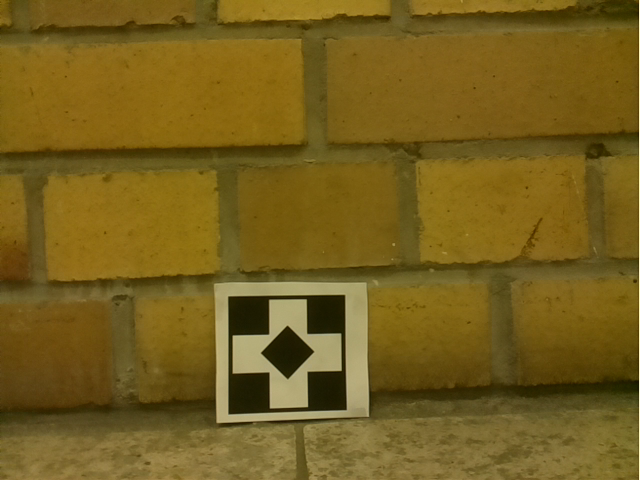
\includegraphics[width=9cm]{img/data1455211246.png}
		\caption{Der Optische Marker den die auf den das Neuronale Netz 
		Trainiert wird. Der Roboter rosBerry wird versuchen den Marker zu 
		finden um ihn anzufahren}
		\label{Marker}
	\end{figure}
	
	Bei Amanda Deckers Bachelorarbeit \cite{Amanda} schien die KI 
	Schwierigkeiten damit zu haben, zwischen dem Marker und einem Blauton 
	zu unterscheiden, der auch im Marker vorkam.
	Es schien auch schwierig zu sein ein Binärbild vom Marker zu erzeugen, 
	da die beiden Farben des Markers einen geringen Kontrast zueinander 
	haben. (Binärbilder enthalten nur die Farben Schwarz und Weiß. Sie 
	entscheiden anhand eines Schwellwerts welche der beiden Farben ein 
	Pixel bekommen wird)
	Da Kameras in OpenCV mit Hilfe von Schachbrettmustern kalibriert werden, wird für dieses Projekt ein Symbol mit ähnlich hohem Kontrast und scharfen Kanten verwendet.
	\\
	
	Dieses Symbol (Abb. \ref{Marker}) ist nicht nur in 4 Richtungen rotierbar, sondern auch zweifach spiegelbar, ohne den Marker zu verfälschen. (Rotationsinvarianz und Spiegelungsinvarianz)
	Es verfügt auch über einen maximalen Kontrast und klare, gerade Kanten.
	\\
	\noindent
	Ein Neuronales Netz kann nur so gut sein wie die Daten, mit denen es 
	trainiert und getestet wurde.
	\\
	Um einen möglichst robusten Datensatz zu bekommen, werden verschiedene Techniken angewendet:
	\begin{itemize}
		\item Um zu verhindern, dass die KI alle Bilder mit starken Kontrasten für einen Marker hält, wird ein Ausschnitt einmal mit und einmal ohne den Marker fotografiert.
		\item Gegen den \glqq schön-wetter KI\grqq-Effekt (eine KI die annimmt jedes gut ausgeleuchtete Bild muss ein Treffer sein) wird der Marker bei verschiedenen Beleuchtungen fotografiert.
		Dazu gehören direktes Sonnenlicht, Schatten, künstliche Beleuchtung mit LED, Lampen und Neonröhren. 
		\item Um zu verhindern, dass die KI alles für ihren Marker hält, was eine gewisse Größe hat und quadratisch ist, wird der Marker aus verschiedenen Distanzen fotografiert. 
		\item Gegen Noise-Anfälligkeit werden verschiedene Hintergründe bei den Fotos verwendet. Teils weiße Wände, teils strukturierte Hintergründe oder eine Freifläche. 
		\item Um zu verhindern, dass sich die KI auf die Bildmitte konzentrieren kann, wird der Marker aus verschieden Positionen fotografiert. 
	\end{itemize}
	
	
	\subsection{Grobübersicht über das System}
	In diesem Kapitel wird zuerst auf die Softwarearchitektur und der 
	Hardwareaufbau von rosBerry eingegangen, danach wird das Software 
	System erklärt.
	
	\begin{figure}[!ht]
		\centering
		\def\svgwidth{9cm}
		\input{img/Gesamtsystem.pdf_tex}
		\caption{Überblick der Komponenten des rosBerry-Softwaresystems}
		\label{Gesamtzusammenhang}
	\end{figure}
	Die Abbildung \ref{Gesamtzusammenhang} zeigt das System, welches auf 
	dem Robot Operating System (ROS) basiert.
	Diese Software läuft verteilt auf den Komponenten Laptop, Raspberry Pi und Arduino.
	\\
	Die Komponente Laptop ermöglicht dem User die Steuerung des 
	Roboters.
	Die Steuerung kann erst erfolgen, wenn auf dem Raspberry Pi ein Accesspoint geöffnet wurde, mit dem sich der Laptop - der Nutzer letztendlich - via WLAN verbindet.
	\\
	Die andere Komponente - der Roboter - besteht aus einem Raspberry Pi und einem Arduino.
	Der Pi ist mit Roscore ausgestattet, auf dem Arduino läuft ein Node für den Ultraschallsensor.
	% ? Besser als das hier: ?
	% Innerhalb der anderen Komponente Roboter - unser rosBerry - befindet sich die beiden Hardware-Elemente Raspberry Pi und ein Arduino. Roscore läuft auf dem Raspberry Pi und ein Node - für den Ultraschallsensor - auf dem Arduino.
	
	Der Arduino wird durch ein USB Kabel mit dem Raspberry Pi verbunden.
	Dadurch wird eine Kommunikation ermöglicht, in welcher der Arduino den Raspberry Pi in Zeitabständen mit Sensordaten versorgt.
	\\
	% Elektronische Bauteile und ihre Funktion
	An dieser Stelle ist anzumerken, dass weitere verwendete Hardware im Kapitel \nameref{sec:Bauteile} näher vorgestellt wird.
	
	%----------------------------------------------------------------
	\subsection{Architektur der ROS-Knoten}\label{sec:Architektur}
	
	%heike
	%grobstruktur,  nodes topics und all das was es schon als text gibt
	In diesem Kapitel wird die Software-Architektur des Roboters vorgestellt.
	%Den dazugehörige Quellcode finden Sie auf https://github.com/Wifi-cable/Robotic\_AI\_student\_project.
	%An dieser Stelle möchten wir darauf hinweisen, dass das Repository von Tiziano Fiorenzani geklont wurde.
	%Die Dokumentation seines Projektes finden Sie unter folgender Verlinkung zu Youtube https://youtu.be/iLiI\_IredhI.
	
	% Das Bild später bei Existenz aller Knoten aktualisieren.
	\begin{figure}[!ht] 
		\centering
		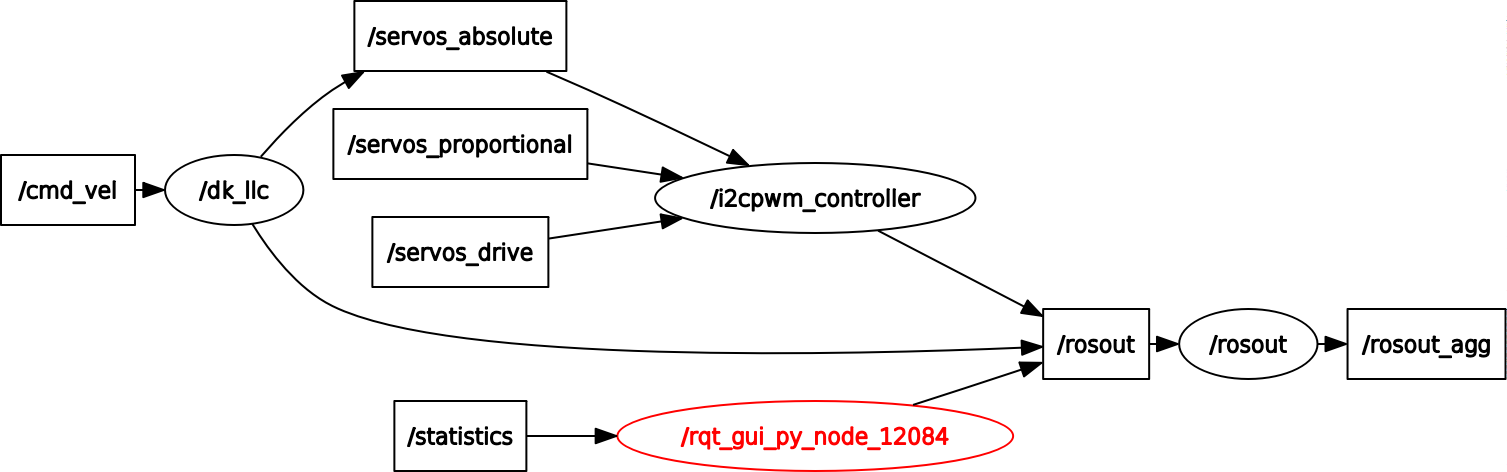
\includegraphics[width=9cm]{img/rosgraph.png}
		\caption{Erste Übersicht der ROS Nodes und Topics innerhalb des rosBerry-Softwaresystems mit Fokus auf die Steuerung des Roboters}
		\label{rosgraph}
	\end{figure}
	
	Treu nach den Prinzipien von ROS besteht die Software aus vielen ROS Nodes, welche als Oval dargestellt werden. 
	Jeder Node erledigt kleine Aufgaben und kann als Subscriber und/oder Publisher fungieren.
	Die Kommunikation zwischen Subscriber und Publisher erfolgt durch ROS Messages (Nachrichten).
	Diese werden durch verschiedene Topics (Themen) kommuniziert, die in den Abbildungen als Rechteck dargestellt werden.
	Die Topics kann man als Kanäle für Nachrichten betrachten.
	
	Folgende Nodes befinden sich im Softwaresystem:
	\begin{itemize}
		\item /rosout (Master)
		\item /teleop\_twist\_keyboard (Fernsteuerung)
		\item /donkey\_llc (Hardwarenahe Steuerung)
		\item /ic2pwm\_board\_node (Bibliothek und Node zum Ansprechen des I2C-Protokolls und deren Verbindung mit ROS)
	\end{itemize}
	
	Die Nodes tauschen Nachrichten über Topics aus.
	Die folgenden Topics befinden sich im Softwaresystem:
	\begin{itemize}
		\item /cmd\_vel (command velocity, die Beschleunigungssteuerung und 
		Lenkung)
		\item /servos\_absolute (Steuerung des Servos mit absoluten Impulsstart- und Stoppwerten)
		\item /servos\_proportional (Motorsteuerung für Geschwindigkeitsteuerung des Servos in seinem Bewegungsbereich)
		\item /servos\_drive (Lenken, Umwandlung der Berechnungen von Linear- und Winkeldaten in Servoantriebsdaten)
		\item /rosout (Standard ROS Output)
	\end{itemize}

	% Hier noch Text zu dem AI Schaubild (kommt noch)
	Die nächste Abbildung veranschaulicht alle Knoten und Topics für die 
	Künstliche Intelligenz. 

	% TODO full width figure (how?)
	\begin{figure}[!ht] 
		\centering
		\def\svgwidth{\linewidth}
		\input{img/AI-Only.pdf_tex}
		\caption{Zweite Übersicht der ROS Nodes und Topics innerhalb des rosBerry-Softwaresystems mit Fokus auf die AI}
		\label{AI-Only}
	\end{figure}

	\begin{itemize}
		\item Auf dem Raspberry Pi befindet sich der Publisher 
		/compress\_sender. Dieser erstellt Fotos mit Hilfe von OpenCV. Im 
		Anschluss werden die Bilder mit Hilfe der CV-Bridge in ROS Bilder 
		umgewandelt und komprimiertet. Die so erstellte ROS Nachricht wird 
		per WLAN über das Topic /camera/image/compressed versendet.
		
		\item Der Node /AI befindet sich auf dem Laptop. Dieser abonniert das 
		komprimierte Bild und wendet darauf das Keras Trainingsmodell an. 
		Nach der Auswertung wird eine String Nachricht über WLAN durch 
		das Topic /Marker an den Node /high\_level\_control versendet. 
		Dieser String enthält eine Richtungsangabe wie \say{Left} oder 
		\say{Forward}. Das Senden über WLAN ist nötig, da sich die  
		/high\_level\_control auf dem Raspberry Pi befindet.
		
		\item Der Publisher /serial\_node wird im Quellcode auf dem Arduino initialisiert. Dieser sendet die erhaltenen Ultraschallsensordaten in kurzen Zeitabständen über das Topic /rngMsg\_topic.
		
		\item Der /high\_level\_controller Knoten abonniert die beiden Topics 
		/Marker und /rangeMsg\_Topic. Er ist für die Steuerung der 
		Geschwindigkeit und der Richtung anhand der KI Daten und der 
		Ultraschallsensordaten zuständig. Der Knoten hat einen Publisher der 
		auf dem  Topic /cmd\_vel (value) eine Geometry/Twist\_Message 
		versendet. So werden Geschwindigkeit und Lenkung des Roboters 
		gesteuert. (angular.z für die Lenkung und linear.x für die 
		Beschleunigung)
		
		
	\end{itemize}

	\subsubsection{Launchreihenfolge}%heike
	
	Dieses Kapitel ist eine Anleitung zum Starten der ROS Nodes. Ohne 
	Vorkonfiguration und Launchfiles ist 
	die Knotenaufrufreihenfolge langwierig. Manche Schritte müssen auf einem 
	Laptop durchgeführt werden, andere via SSH auf dem Raspberry Pi. So 
	muss der Laptop erfahren das ein ROScore (Master Node) bereits auf dem 
	Raspberry Pi läuft.
	
\begin{figure}
	\centering
\begin{minted}[frame=lines, breaklines=true 
fontsize=\footnotesize,]{Bash}
# Network ubiquityrobot03B
# connect via SSH
ssh ubuntu@10.42.0.1
# enter password
	
# 1. Console - on Raspberry Pi
# Login via SSH
cd catkin_ws/Robotic_AI_student_project/
# If bash.rc wasn't changed to source workspace
source devel/setup.bash
rosrun i2cpwm_board i2cpwm_board
	
# 2. Console - on Raspberry Pi
# Login via SSH
cd catkin_ws/Robotic_AI_student_project/
source devel/setup.bash
rosrun donkey_car low_level_control.py
	
# 3. Console - on Laptop 
export ROS_MASTER_URI=http://ubiquityrobot.local:11311
export ROS_IP=$(hostname -I)
cd catkin_ws/Robotic_AI_student_project/
source devel/setup.bash
rosrun teleop_twist_keyboard teleop_twist_keyboard.py
	
# 5. Console - on Laptop
export ROS_MASTER_URI=http://ubiquityrobot.local:11311
export ROS_IP=$(hostname -I)
	
	\end{minted}
	\label{StartNodes}
	\caption{Start der Nodes ohne Verwendung einer veränderten 
	bash.rc-File. Zuerst wird eine Verbindung zum Raspberry Pi via SSH 
	hergestellt. In jeweils unterschiedlichen Konsolen werden die beiden 
	Nodes i2cpwm\_board - eine Node zum Ansprechen des I2C-Protokolls und 
	deren Verbindung mit ROS - und low\_level\_control - die hardwarenahe 
	Steuerung - gestartet.}
\end{figure}
	
	Mehrere Schritte sind möglich um diesen Prozess zu vereinfachen. Die 
	meisten Optionen sind eine Frage der persönlichen Präferenz des ROS 
	Benutzers. So kann ein Eintrag in die systemweit geltende Datei 
	\textit{bash.rc} die Eingabe von \textit{source devel/setup.bash} im ROS 
	workspace ersetzen. \\
	Eine weitere Erleichterung ist der Eintrag eines Shellscripts in die 
	setup.bash Datei. \ref{Einzeiler} Dieser Eintrag setzt die ROS Host IP 
	Variable auf die aktuelle IP Adresse des Laptops.
	\begin{figure}
		\centering
\begin{minted}[frame=lines,breaklines=true,
fontsize=\footnotesize,
framesep=2mm
]{Bash}
export ROS_IP=$(ip -br -4 address show dev wlp3s0 | awk '{print $3}' | 
awk -F '/' '{print $1}')
\end{minted}
		\label{Einzeiler}
		\caption{Arbeitserleichterung damit zwei ROS Rechner mit einander 
		kommunizieren können: ROS-IP - Verbindung via SSH - mittels Bash 
		Einzeiler setzen  in der setup.bash (Autor J.K.)}
	\end{figure}
	\\
	Eine weitere Möglichkeit der Vereinfachung besteht im Erstellen von 
	SSH-Keys. 
	
	\subsubsection{Launchfiles}
	
	Launchfiles, die viele ROS Knoten auf einmal starten, sind eine beliebte 
	Vereinfachung. Um die \textit{Keyboard Demo} \ref{demo} zu starten, oder 
	den Roboter Fernzusteuern existiert ein Lauchfile im \textit{Donkey Car} 
	Fork der Github Quelle.
	\begin{figure}
		\centering
\begin{minted}[frame=lines,breaklines=true,
fontsize=\footnotesize,
framesep=2mm
]{Bash}
#call on Raspberry Pi to launch hardware nodes
roslaunch donkey_car keyboard_demo.launch
#call keyboard node from laptop 
rosrun teleop_twist_keyboard teleop_twist_keyboard.py
\end{minted}
\label{demo}
\caption{Launchfile aufrufe um den Roboter per Tastatur vom Laptop aus 
 Raspberry Pi keyboard\_demo\_launch und auf dem Laptop 
 teleop\_twist\_keyboard gestartet werden.}

	\end{figure}
	
	Um die benötigten Knoten Für die Künstliche Intelligenz komfortabel zu 
	starten wurden zwei Launchfiles geschrieben \ref{KI-launch}. Das ist 
	notwendig da die Anwendung verteilt läuft. (siehe spätere Artikel)
	
	\begin{figure}[h]
		\centering
\begin{minted}[frame=lines,breaklines=true,
fontsize=\footnotesize,
framesep=2mm
]{Bash}
#call from Raspberry Pi
roslaunch donkey_car hardware.launch
#call from Laptop
export ROS_MASTER_URI=http://ubiquityrobot.local:11311
roslaunch ki_nav start_AI.launch
		\end{minted}
		\label{KI-launch}
		\caption{Künstliche Intelligenz, oder Autonomes verhalten, auf Laptop 
		und Raspberry Pi starten per Launchfile }
	\end{figure}
	%----------------------------------------------------------------
	
	\section{Praktische Projektdurchführung}
	
	%----------------------------------------------------------------
	
	In diesem Kapitel wird der Hardwareaufbau des rosBerry, sowie die 
	mechanischen Bauteile beschrieben. Zusätzlich wird auf einige 
	Entscheidungskriterien für die Auswahl von Bauteilen eingegangen. 
	Hierfür werden die einzelnen verwendeten Hardwarekomponenten - deren Modell und Funktion - vorgestellt. 
	
	Zuerst werden die Verbindungen der Hardwarekomponenten untereinander abgebildet, wie in Abbildung \ref{Hardwarekomponenten} zu sehen.
	\subsection{Mechanische Bauteile}
	
	\begin{figure}[h]
		\centering
		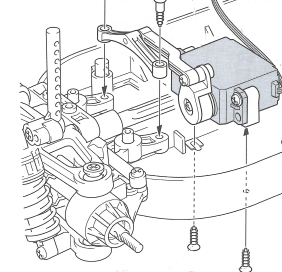
\includegraphics[width=9cm]{img/servo.pdf}
		\caption{Auszug aus Hersteller Datenblatt, wie die Lenkstange am 
		Servomotor  befestigt ist. Dieser Servo einer von zwei Motoren, er  ist 
		Jedoch alleine für die Lenkung zuständig. }
		\label{Servomotor}
	\end{figure}
	Für das Robotik Projekt \textit{rosBerry} wurde ein solides, aber günstiges Chassis gesucht bei dem die Möglichkeit besteht Ersatzteile zu bestellen. Viele qualitativ hochwertige Modellbau Chassis liegen in einem Preisrahmen über 400€, für diese ist die Ersatzteilbeschaffung gut möglich. Günstige, meist asiatische Modellbau Chassis Hersteller liefern ihre Modelle und Bausätze nur für einen kurzen Zeitraum. Es ist oft nicht möglich zu einem späteren Zeitpunkt das Modell nachzukaufen oder Ersatzteile zu bekommen. Somit ist ein Roboter der darauf aufbaut, wie das Donkey Car, nicht reproduzierbar. 
	\\
	\begin{figure} %[t]
		\centering
		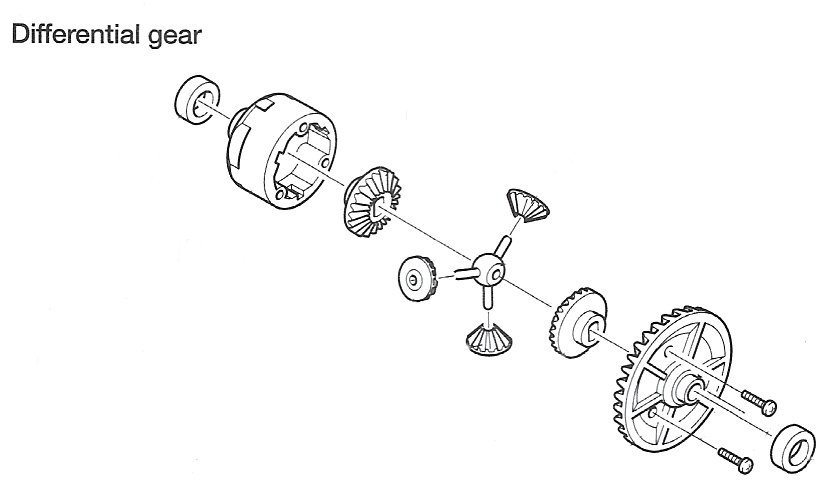
\includegraphics[width=9cm]{img/geer.png}
		\caption{Auszug aus Hersteller Datenblatt: Differnzialgetriebe. Auch 
		wenn der Roboter Differnzialgetriebe hat, ist die Lenkung eine 
		Akkermann Lenkung. Der Roboter hat keine Differenzial Lenkung da 
		ein Motor ausschließlich für den Vorschub zuständig ist. }
		\label{Getriebe}
	\end{figure}
	Der Kompromiss dieser Abwägung fand sich bei einem älteren 
	Einsteigermodell namens TAMIYA RC 1:10 TT-01E. Tamiya ist ein 
	traditionsreicher japanischer Hersteller der qualitativ hochwertige 
	Bausätze für ferngesteuerte Fahrzeuge herstellt. (Er stellt Schiffe, Flugzeuge 
	und Panzer her, aber hauptsächlich Modellautos) Tamiya ist unter 
	Modellbau-Enthusiasten dafür bekannt, alle Prinzipien japanischer 
	Ingenieurskunst bei der Konstruktion seiner Modelle anzuwenden, statt 
	\say{Spielzeugqualität} in China herzustellen. Das TT01-Modell hat 
	identische Außenmaße und kann mit denselben elektronischen Komponenten 
	betrieben werden wie sein Nachfolgemodell TT02. Somit ist die 
	Reproduzierbarkeit im Bezug auf das Chassis gegeben.
	\\
	Die Mechanik des \textit{TAMIYA RC 1:10 TT-01E } Modells basiert auf 
	einem Motor und einer langen Antriebswelle, die drei Differenzialgetriebe 
	bewegt. \ref{Getriebe} Die Modelle werden als Vierradantrieb vermarktet. 
	Die Lenkung wird getrennt vom Antrieb durch einen kleinen Servomotor 
	geregelt\ref{Servomotor}. Er bewegt die Spurstange nach rechts / links. Das 
	Chassis nutzt also eine Ackermann Lenkung, wie sie auch bei PKWs üblich ist.
	
	\subsection{Elektronische Bauteile und ihre Funktion}\label{sec:Bauteile}
	% SVG ?
	\begin{figure} %[t]
		\centering
		\def\svgwidth{9cm}
		\input{img/Hardwarekomponenten.pdf_tex}
		\caption{Verwendete Hardwarekomponenten und deren Verbindungen untereinander im rosBerry}
		\label{Hardwarekomponenten}
	\end{figure}
	
	Wie in Abbildung \ref{Hardwarekomponenten} zu erkennen, ist die meiste Hardware mit Jumper Wire verbunden.
	Ausnahmen bilden die Verbindungen des Raspberry Pi's 
	zur Kamera (Flexkabel), zum Arduino (USB) und zum Motorshield (I2C).
	\\
	
	%Als Nächstes wird rosBerry mit den Hardwaremodellen vorgestellt.
	
	\begin{figure}[!ht]
		\centering
		\includegraphics[width=9cm]{img/RosBerryGesamt_yellow.png}
		\caption{Übersicht der Position der Hardware - DC-Antriebsmotor, Fahrtenregler, UBEC, Servo, Akku, Motorshield, Raspberry Pi und Arduino - im rosBerry}
		\label{rosBerryGesamt}
	\end{figure}
	
	Die verwendete Hardware ist in Abbildung \ref{rosBerryGesamt} mit Nummern versehen.
	Auf jede dieser Nummern wird referenziert und der Hardwaretyp und 
	seine Funktion aufgelistet.
	
	\begin{enumerate}
		\item Der DC-Antriebsmotor - Modell Tamiya Mabuchi RS 540 SH - steuert alle vier Räder des rosBerry an.
		Ohne ihn wird der Roboter nicht in Bewegung kommen.
		\item Neben dem DC Antriebsmotor befindet sich ein Fahrtenregler, Modell BORSTI 1/10 BRUSHED-ESC 45A.
		Dieser erhält vom Motorshield ein PWM-Signal, welches er verstärkt.
		Das verstärkte PWM-Signal wird anschließend in Geschwindigkeit umgesetzt und an den DC-Antriebsmotor weitergeleitet.
		\item Der UBEC - Modell HWBEC Hobbywing 3A \SI{5}{V} \SI{6}{V} max \SI{5}{A} - wird eingebaut, um den Raspberry Pi mit \SI{5}{V} zu versorgen.
		Ohne den UBEC würde der Raspberry Pi aufgrund der höheren elektrischen Spannung beschädigt werden.
		\item Der Servo - Modell Amewi AMX Racing 4806HB - bekommt vom Motorshield ein PWM Signal übermittelt.
		Nach dem PWM Signal richten sich die beiden Vorderräder aus.
		Dadurch ist rosBerry in der Lage links\,/\,rechts Kurven sowie geradeaus zu fahren.
		\item Der Akku dient dazu, die Stromversorgung des Roboters zu sichern.
		Dieser hat eine Nennspannung von \SI{7,2}{Volt}. 
		\item Der Motorshield - Modell Adafruit 16-Channel 12-bit PWM/Servo 
		Driver-I\textsuperscript{2}C interface PCA9685 - wird für die 
		Motorsteuerung eingesetzt.
		Hierzu erzeugt der Motorshield zwei PWM Signale.
		Das 1. PWM Signal wird an den Servo übermittelt, um den Servo in die 
		gewünschte Position drehen.
		Das 2. PWM Signal wird zum Fahrtenregler gesendet.
		Dadurch wird die Geschwindigkeit geregelt.
		\item Der Raspberry Pi 3 B+ ist das Herzstück des rosBerry.
		Auf ihn läuft zum einen ROS und zum anderen die Software des Roboters, welche im Kapitel \nameref{sec:Architektur} vorgestellt wird.
		Über eine I\textsuperscript{2}C-Schnittstelle werden Daten an den 
		Motorshield übertragen.
		Die Daten geben an, wie das PWM Signal auszusehen hat.
		\item Der Arduino UNO steuert einen Ultraschallsensor an und erzeugt 
		einen ROS-Knoten (Publisher).
		Innerhalb des Programms wird das Signal des Sensors in Meter umgewandelt und in eine Range Message gespeichert.
		Die Range Message namens rangeMsg wird an das Topic rangeMsg\_topic übermittelt.
		Ein Subscriber, der auf dem Raspberry Pi läuft, abonniert das Topic und erhält regelmäßig Sensordaten über die Reichweite.
		
		\begin{figure}
			\centering
			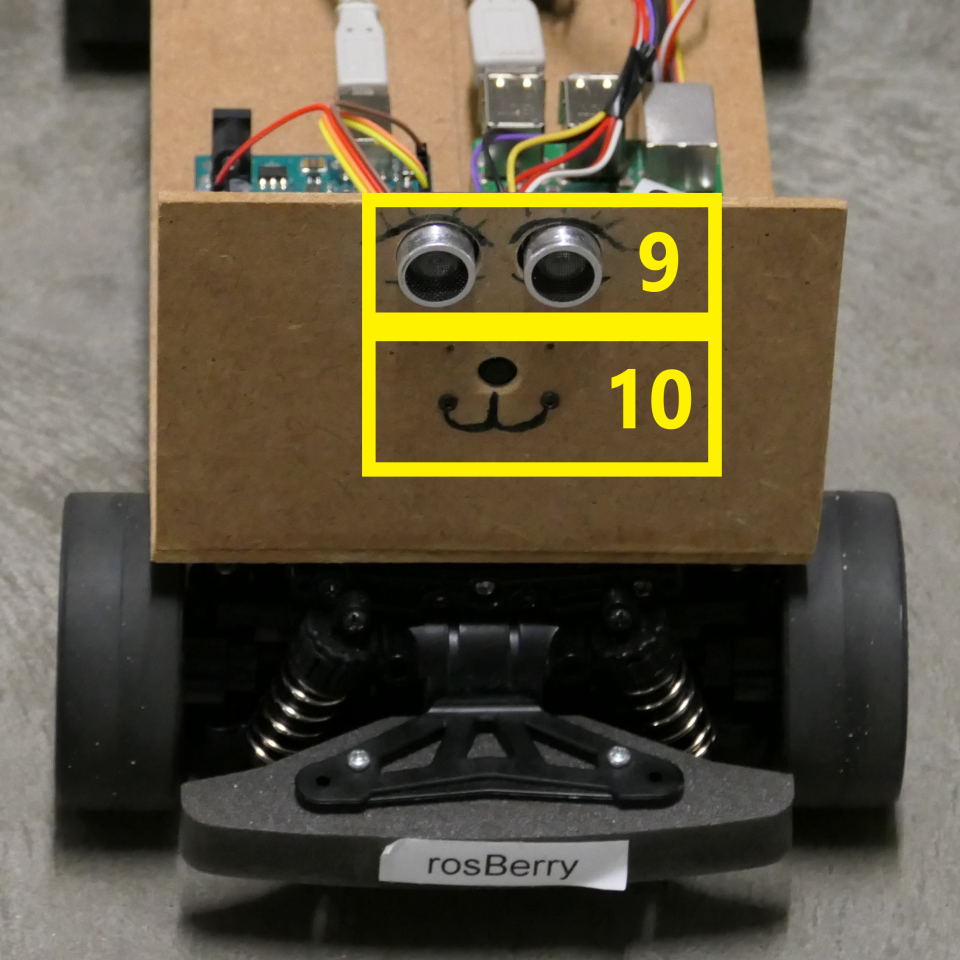
\includegraphics[width=5.5cm]{img/RosBerryWeitere_yellow.png}
			\caption{Position der Kamera und des Ultraschallsensors im rosBerry}
			\label{rosBerryWeitere}
		\end{figure}
		\item Der Ultraschallsensor - Modell HC-SR04 - wird zum rechtzeitigen 
		Erkennen von Hindernissen eingesetzt.
		Dieser hat eine maximale Reichweite von vier Metern.
		Alle ¼ Sekunde sendet dieser ein Signal und verarbeitet dieses.
		\item Die Kamera - Modell 5 MP - ist durch ein Flexkabel an den Raspberry Pi über das CSI-Interface angeschlossen.
		Diese versorgt die KI mit Bildern, welche einen Marker sucht und findet.
	\end{enumerate}
	
	%----------------------------------------------------------------
	
	
	\section{Autonomes Verhalten durch Künstliche Intelligenz}	%mary
	
	Ziel des KI-Teils des Projektes besteht darin, dem Roboter beizubringen, einem optischen Marker zu folgen.
	Dazu muss er erst einmal das Symbol erkennen, dann herausfinden in welcher Richtung sich der Marker befindet.
	Danach erst kann er auf den Marker zufahren.
	\\
	
	Dazu muss der Marker zuverlässig in unterschiedlichen Umgebungen 
	erkannt werden.
	
	\subsection{Erster Ansatz für das Neuronale Netz}	%steffen ? mary?

	Der erste Entwurf unseres Neuronalen Netzes ist stark angelehnt an F. Grovers Beispielnetz aus \glqq Artificial Intelligence for Robotics\grqq \cite{govers2018artificial}. 
	Wie in der Vorlage wird ein sequentielles Modell mithilfe von Keras 
	erstellt.
	
	Die erste Schicht stellt eine Convolution-Layer mit 20 Convolutions dar, 
	wovon jede ein Merkmal des Eingangsbildes isolieren soll.
	Die Größe wird auf 5x5 gesetzt, betrachtet also zwei benachbarte Pixel in 
	jede Richtung.
	Selbstverständlich muss dafür auch ein Padding hinzugefügt werden, damit das Verfahren auch am Bildrand funktioniert. 
	
	Zudem wird noch eine Aktivierungsfunktion benötigt, in diesem Fall  die 
	ReLU-Funktion, die nur positive Werte zulässt und negative Werte durch 
	den Wert 0 ersetzt.
	Diese Aktivierungsfunktion ist deshalb sinnvoll, da das Ergebnis als 
	Farbpixel dargestellt werden und deshalb einen Wert zwischen 0 und 1 
	annehmen soll.
	Ein Wert unter Null wäre hier unbrauchbar.
	
	\begin{figure}[!h]
		\centering
		\begin{minted}[frame=lines]{Python}
model = Sequential()
inputShape = (height, width, depth)

model.add(Conv2D(20, (5, 5), padding="same", input_shape=inputShape))
model.add(Activation("relu"))
		\end{minted}
		\caption{Modell: erste Schicht}
		\label{Schicht eins}
	\end{figure}
	
	Die zweite Schicht ist ein Maxpooling-Layer, bei der jeweils 2x2 Pixel 
	genommen werden und danach 2x2 Pixel weiter gerückt wird, um keine 
	Überlappungen zu haben.
	Das Ergebnis ist ein Bild in ¼ der originalen Größe: aus 640x480px wird 320x240px, aus 128x128px 64x64px usw.
	
	Direkt darauf folgt eine weiteres Convolution Layer mit der doppelten 
	Anzahl an Convolutions - 40 statt vorher 20 - um mehr Merkmale zu 
	identifizieren.
	Durch das vorher durchgeführte Maxpooling werden nun andere, größere Merkmale erkannt.
	 Dieselbe ReLU Aktivierungsfunktion wird genutzt, aus denselben 
	 Gründen wie in der ersten Schicht.
	
	\begin{figure}[!h]
		\centering
		\begin{minted}[frame=lines]{Python}
model.add(MaxPooling2D(pool_size=(2, 2), strides=(2, 2)))
model.add(Conv2D(40, (5, 5), padding="same"))
model.add(Activation("relu"))
		\end{minted}
		\caption{Modell: zweite und dritte Schicht}
		\label{Schicht zwei und drei}
	\end{figure}
	
	%\begin{lstlisting}[label={list:model_1_2},caption=Modell: zweite und dritte Schicht]
	%	model.add(MaxPooling2D(pool_size=(2, 2), strides=(2, 2)))
	
	%	model.add(Conv2D(40, (5, 5), padding="same"))
	%	model.add(Activation("relu"))
	%\end{lstlisting}
	
	Schicht vier besteht erneut aus einem Maxpooling-Layer, ebenfalls um nochmals größere Merkmale zu erkennen.
	Aus einem 640x480px großen Bild wird nun 160x120px, aus 128x128px sogar nur noch 32x32px.
	
	Darauf folgt nun eine Schicht, die vorher noch nicht im Neuronalen Netz vorkam:
	Zuerst werden die dreidimensionalen Bildinformationen mit der Funktion 
	Flatten() in ein eindimensionales Array geplättet, bevor eine 
	vollverknüpfte Schicht mittels Dense(500) hinzufügt wird.
	Erneut wird die ReLU Aktivierungsfunktion genutzt, aus bekannten 
	Gründen.
	
	\begin{figure}[!h]
		\centering
		\begin{minted}[frame=lines]{Python}
model.add(MaxPooling2D(pool_size=(2, 2), strides=(2, 2)))

model.add(Flatten())
model.add(Dense(500))
model.add(Activation("relu"))
		\end{minted}
		\caption{Modell: vierte und fünfte Schicht}
		\label{Schicht vier und fünf}
	\end{figure}
	
	Abschließend werden zwei Neuronen für die beiden Ausgangswerte 
	"Marker"\ und "kein Marker"\ benötigt.
	Zur Aktivierung wird die Softmax-Funktion genutzt, die auch 
	normalisierte Exponentialfunktion genannt wird.
	Sie transformiert mehrdimensionale Vektoren in einen Wertebereich zwischen 0 und 1, wobei alle Komponenten zusammen 1 ergeben müssen, das heißt wenn "Marker"\ einen Wert von 0,65 hat, muss "kein Marker"\ einen Wert von 0,35 haben. 
	Die Funktion kann durchaus für mehr als zwei Ausgangswerte genutzt werden, für unseren Anwendungsfall werden jedoch nicht mehr Ausgangswerte benötigt.
	
	\begin{figure}[!h]
		\centering
		\begin{minted}[frame=lines]{Python}
model.add(Dense(2))
model.add(Activation("softmax"))
		\end{minted}
		\caption{Modell: finale sechste Schicht}
		\label{Schicht sechs}
	\end{figure}

	\subsubsection{Erste Auswertung der Ergebnisse}	%steffen? 
	%wiso war das scheisse 
	%weil wir einfach das Beispiel aus dem Buch kopiert haben…

\begin{figure}[!h]
	\centering
	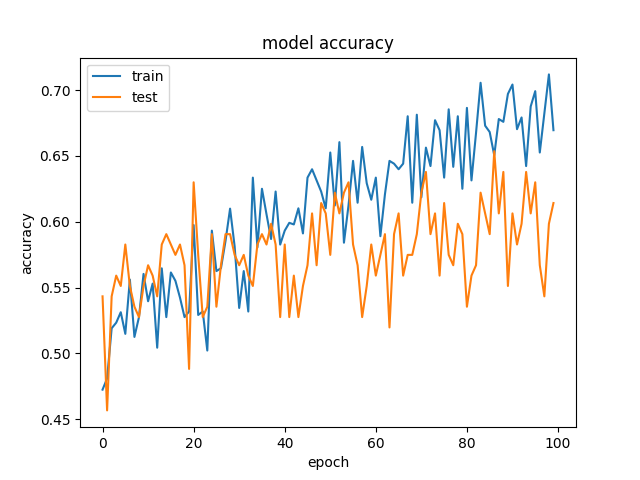
\includegraphics[width=9cm]{img/160x120:100@32_accuracy.png}
	\caption{Zweiter Durchlauf des Neuronalen Netzes mit dem Beispiel 
		Code des Buches, Ausgangszustand vor Verbesserungsmaßnahmen. Die 
		Blauen Trainingsdaten steigen langsam gegen 
		70\%. Die Orange Kurve der Valiedierungsdaten jedoch läuft schon 
		nach rund 50 Epochen deutlich Flacher. }
	\label{Initiales Ergebnis}
\end{figure}
Beim ersten Durchlauf des Neuronalen Netzes ist die Erkennungsrate des 
Markers 57\%. Dieses Ergebnis ist bei einer 50/50 Chance kaum besser als 
Raten. Beim zweiten versuch mit mehr Durchläufen (Epochen) ist das 
Ergebnis nur Unwesentlich besser. Das Overfitting , oder das 
auseinanderlaufen der Trainings und Validierung kurve ist schnell sichtbar. 
Ein Auseinanderlaufen bedeutet, dass die KI ihr Modell zu sehr auf ihre 
Trainingsdaten angepasst hat. Sie kommt schneidet mit anderen Testdaten 
schlechter ab als mit den Daten auf denen Sie trainiert wurde. 


	\subsection{Schritte zur Verbesserung der Erkennungsrate} %mary
Da diese Ergebniss wenig befriedigend ist wird ein leicht veränderter Ansatz 
benötigt. \\
	Die Schritte von \glqq Learn Keras for Deep Neural Networkss\grqq \cite{moolayil2019learn} zum Verbessern des Designs von Neurnalen Netzen werden zur verbesserung der Trainignsergebnisse verwendet. 
	
	\cite{moolayil2019learn} rät dazu mit einer kleinen Architektur anzufangen,
	dass bedeutet wenige Schichten und eine geringe Anzahl an Neuronen. Es 
	liegt nahe, dass kleine Architekturen ressourcenschonender sind als 
	grosse Architekturen. Dieser Ansatz erscheint sinnvoll, da steigende 
	Resourcenanforderngen bei gleichbleibender Hardware zu steigender 
	Rechenzeit pro Epoche führen. \\
	
	Das Netz nutzt anfangs nur eine Auflösung von 128x128 Pixel und 100 
	Epochen. Da jedes einzelne Pixel eine Eingangsneurone wird, ist 
	anzunehmen, dass die geringe Auflösung im Buch 
	\cite{govers2018artificial} gewählt wird, um Rechenleistung zu 
	sparen. \\
	

	
	\cite{moolayil2019learn} rät die Anzahl an Neuronen pro Schicht erhöhen, wenn Anfangs keine befriedigenden Ergebnisse erzielt werden.
	Bei voller Bildauflösung von 640x480 Pixel erweist sich das Neuronale 
	Netz auf der Hardware eines handelsüblichen Laptops als nicht mehr 
	lauffähig. Für weitere Durchläufe wurden die nächsten Versuche auf einer 
	Workstation mit mehr Grafikkarten und deutlich mehr RAM gemacht. 
	Die Erkennungsrate steigt bei größerer Auflösung und mehr Durchläufen 
	tatsächlich auf über 80\%. Damit vergrössert sich jedoch auch das Modell (die 
	Gewichte der KI) auf über ein Gigabyte. Ein so großes Modell kann nicht 
	zeitnah auf einem Raspberry Pi angewedet werden, da es nicht mehr in 
	den RAM passt. Auch auf Standard Laptops ist zu erwarten, dass ein 
	größeres Modell Berechnungen in Echtzeit erschwert. \\
	
	Um mit einer höheren Auflösung trainieren zu können werden die 
	nächsten Trainingseinheiten auf einem performanteren Server 
	durchgeführt. Der zusätzliche Arbeitsspeicher und die Grafikarten 
	bringen bei einer Aktivierung der CUDA Beschleunigung einen großen 
	Geschwindigkeitszuwachs. \\
	
	Ein weiteres Problem, dass nun aufkommt ist das Overfitting. Das Modell entwickelte sich gut auf Trainingsdaten, schneidet jedoch deutlich schlechter bei Testdaten ab, mit denen es nicht trainiert hatte. Die Kurven laufen bei mehr als 200 Epochen weit auseinander.\\
	
	\begin{figure}[!h]
	\centering
	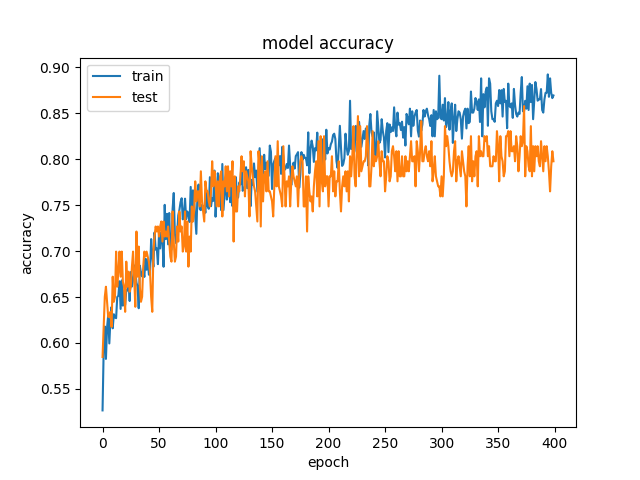
\includegraphics[width=9cm]{img/213x160:400@32_accuracy.png}
	\caption{Deutlich späteres Overfitting, bei Höherer Bildauflösung, zu dem 
	Preis von deutlich höhere Rechenzeit pro Epoche. Erste Dropout Schicht 
	wurde eingeführt. }
	\label{Overfitt }
\end{figure}
	Weiterhin rät \cite{moolayil2019learn} mehr Schichten zu benutzen, 
	beispielsweise abwechselnd eine dichte Schicht (dense layer) und eine 
	Dropout Schicht.
	
	Dropout Schichten im Neuronalen Netz verbessern das Overfitting 
	Problem. Somit sind mehr Trainingsläufe ohne Overfitting möglich. Das 
	neuronale Netz erreicht so Werte von rund 85\%. \\
	
	Das TensorFlow / Keras Modell, dass bei voller Auflösung oder 307200 
	Eingangsneuronen erstellt wird, hat eine Größe von über einem 
	Gigabyte. Je größer das Modell ist, desto unwahrscheinlicher, dass ein 
	Raspberry Pi das Modell in absehbarer Zeit auf ein Bild anwenden kann. 
	Somit erweist sich der Ansatz, einfach die Auflösung zu erhöhen, nicht als 
	zielführend für den Anwendungsfall. \\
	
	Das Modell muss also kleiner werden, ohne wesentliches Overfitting. 
	Dieses Ziel wird durch die Kombination von Dropoutschichten, mehr 
	Durchläufen und kleinerer Pixelanzahl erreicht. \\
		\begin{figure}[!t]
		\centering
		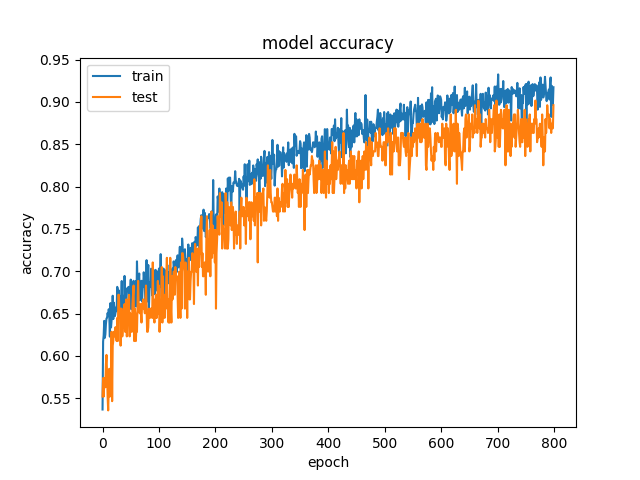
\includegraphics[width=9cm]{img/213x160:800@32:0_accuracy.png}
		\caption{Endergebnis, nach Nachbesserung des Datensatzes, Dropout 
		Schichten und leicht erhöhter Auflösung von 213 x 160 Pixel}
		\label{end Ergenisse }
	\end{figure}
	 Wenn eine Steigerung der Anzahl an Schichten und der Neuronen keine 
	 weitere Steigerung der Erkennungsrate bringt, rät der Autor in 
	 \cite{moolayil2019learn} die Daten neu zu analysieren. Es werden also 
	 Bilder mit sehr geringem Kontrast aussortiert, ebenso extrem dunkle Bilder 
	 sowie Bilder auf denen der Marker sehr weit entfernt war. Sie werden 
	 durch bessere Daten ersetzt, indem neue Bilder je mit und ohne Marker angefertigt werden.
	 Dieser Schritt verursacht eine merkliche Verbesserung des Trainingsergebnis.
	\\
		

	Alle weiteren Versuche, dass Modell weiter zu Verfeinern scheitern. Die 
	Ursache dafür ist nicht eindeutig geklärt, möglich ist aber, 
	dass der Datensatz für die Komplexität des Modells zu klein ist. Auch 
	kann es sein, dass die Grenzen der Optimierer ADAM und Stochastic 
	Gradient Descent erreicht sind. Auch Programmierfehler können nicht 
	ausgeschlossen werden. 
	
	\begin{figure}[!h]
		\centering
		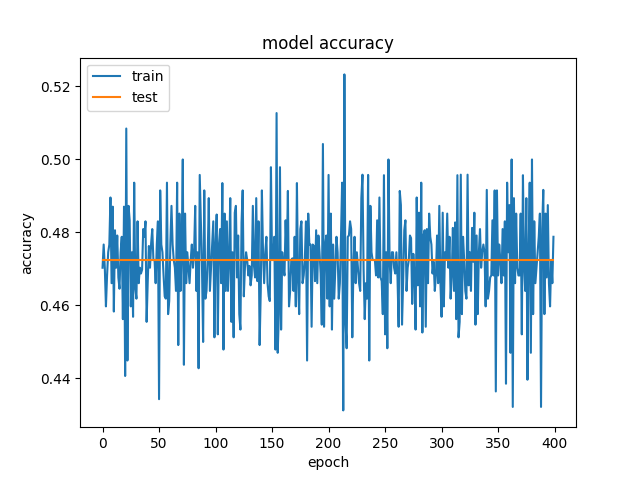
\includegraphics[width=9cm]{img/480x360:400@32_accuracy.png}
		\caption{Kein sichtbarer Trainingserfolg, Grenzen des Optimierers 
		erreicht}
		\label{erfolgloos }
	\end{figure}
	
	
	\subsection{Anwendung des Trainingsmodells} %steffen
	Zu diesem Kapitel gehört der Versuch ein Keras Modell auf einem 
	Raspberry Pi auszuführen, die Technischen Herausforderungen, im 
	Zusammenhang mit ROS  die verwendeten Algorithmen sowie ihr Effekt. 
	
	\subsubsection{Keras und Tensorflow auf Raspberry Pi Hardware}
	Der initiale Plan sieht vor, dass das neuronale Netz auf dem Raspberry Pi 
	ausgewertet wird, damit der Roboter komplett autonom (ohne WLAN und 
	externen Computer) fahren kann. Die Prozessorleistung und der RAM 
	eines Raspberry Pi's 3 B+ ist zwar deutlich geringer als der eines 
	Standard Laptops, aber die Nachteile eines verteilten Systems erscheinen 
	anfangs größer. Besonders der architektonische Aufwand für verteilte 
	Systeme und das Einarbeiten in die Bibliothek CV Bridge zum Versenden 
	von Bildern per ROS Topic wirkt aufwendig. \\
	Die meisten gängigen Bibliotheken und Frameworks sind unabhängig vom 
	Zielbetriebssystem auf 64Bit Wortbreite ausgelegt, so auch Tensorflow 
	und Keras. Das verwendete Ubuntu Image mit ROS für Raspberry Pi 
	jedoch ist ein 32 Bit System. Das bedeutet, es gibt keine vorkompilierten 
	Versionen von Tensorflow für das bisherige Setup. Das Kompilieren 
	großer Tarfiles auf einem Raspberry Pi dauert oft länger als eine Stunde. 
	Teilweise läuft der Raspberry Pi dabei so heiß, dass er abstürzt. Ein 
	externer Ventilator erweist sich hier als hilfreich. Da Tensorflow eine große 
	Bibliothek ist, wäre ihre Kompilierung aufwendig.
Q-engineering	\cite{qengineering}
	Sagt über den Raspberry Pi 4: \\
	\say{The whole TensorFlow installation procedure from start to end takes 
	many hours (±33 for Python, ±10 for the C++ library). } \\
	Übersetzt bedeutet das, dass der komplette Tensorflow Installationsprozess von Anfang bis Ende viele Stunden benötigt. Für Python rund 33 Stunden, für die C++ 
	Bibliothek rund 10 Stunden.
	Es ist anzunehmen, dass der Zeitaufwand für eine Kompilierung auf dem 
	weniger performanten Raspberry 3 B länger dauert. Da es keine Garantie 
	gibt, dass Bibliotheken die für 64 Bit Systeme geschrieben wurden, auch 
	auf 32 Bit Systemen reibungslos funktionieren, ist eine Kompilierzeit 
	von über einem Tag nicht akzeptabel. \\
	
Somit wird die Entscheidung für ein verteiltes System getroffen. Dabei 
zeigen sich weitere erwähnenswerte Inkompatibilitäten. Für jede ROS 
Version (Distribution) existieren vorgepackte Installationspakete für ein 
Ubuntu Betriebssystem. Nur mit diesem System sind sie komplett 
kompatibel. Das Betriebssystem Ubuntu 18.04 ist mit ROS Melodic 
vorgesehen. Während das Betriebssystem Python 2.7 und Python 3.6.9. 
nutzt ist ROS Melodic auf Python 2.7 angewiesen. Die Python Versionen sind 
inkompatibel. Tensorflow2 benötigt eine aktuelle Python Version, die von 
ROS Melodic nicht ohne Weiteres unterstützt wird. \\

Tensorflow1 ist zwar mit Python 2.7 kompatibel, es ist jedoch nicht 
threadsafe. Das scheint anfangs kein Problem zu sein, da keine parallele 
	Programmierung geplant ist. Ein Prototyp-Programm mit Anwendung vom 
	neuronalem Netz läuft problemlos auf Mac mit Python 3 (ohne ROS 
	Publisher und Subscriber). Dieses Programm 
	soll als Vorlage für einen ROS Knoten dienen. Auf Ubuntu in ROS treten 
	jedoch viele kryptische Fehlermeldungen auf. (Abb. \ref{Error1}, Abb. \ref{Error2}, Abb. \ref{Error3}) 
	Die Tatsache, dass die Fehlermeldungen beim Durchlauf eines 
	unveränderten Programms unterschiedlich sind, verwirrte anfangs. 
	Nicht deterministisches Verhalten deutet entweder auf Zufall hin, 
	oder auf Probleme bei der Parallelen Ausführung. 
	
	\begin{figure}
		\centering
		\begin{minted}[frame=lines,
fontsize=\footnotesize,
framesep=2mm]{Bash}
Not found: Container localhost does not exist. 
(Could not find resource: localhost/conv2d_2/kernel)
[[{{node conv2d_2/Conv2D/ReadVariableOp}}]]
\end{minted}
		\label{Error1}
		\caption{Fehlermeldung: Localhost existiert nicht, bei regulärem 
		Aufruf 
		des Keras Modells}
	\end{figure}
	
	\begin{figure}
		\centering
		\begin{minted}[frame=lines,
fontsize=\footnotesize,
framesep=2mm]{Bash}
InvalidArgumentError: Tensor 
dropout__input:0, specified in either 
feed_devices or fetch_devices
was not found in the Graph
		\end{minted}
		\label{Error2}
		\caption{Unverständliche Fehlermeldung, bei regulärem Aufruf 
			des Keras Modells}
	\end{figure}
		
	\begin{figure}
		\centering
		\begin{minted}[frame=lines,
fontsize=\footnotesize,
framesep=2mm]{Bash}

ValueError: Tensor Tensor
("activation_5/Softmax:0",
shape=(?, 2), dtype=float32) 
is not an element of this graph.
\end{minted}
		\label{Error3}
		\caption{Tensorflow Graphenelement unbekannt, eine weitere 
		Fehlermeldung bei nicht Threadsavem Aufruf von Keras Modell}
	\end{figure}
	
	Es hat sich herausgestellt, dass entweder ROS, Python, Tensorflow oder die Kernel 
	des Betriebssystems den Bildanalyse-Algorithmus als hochgradig 
	parallelisierbar erkannt hat. Der Algorithmus im ROS Knoten nutzt mehr 
	als einen Thread bei der Ausführung um die Mehrkern CPU auszunutzen. 
	Die abschließende Ursache kann zum Zeitpunkt des Papers nicht geklärt 
	werden.
	Laut Victor Meunier's Blog \cite{Keras} 
	muss sichergestellt werden, dass jeder Thread seinen eigenen Graphen und seinen eigene Session hat. Das Schlüsselwort \say{With} hilft den Kontext zu definieren. [\ref{with}]\\
	
	\begin{figure}
		\centering
		\begin{minted}[frame=lines,
fontsize=\footnotesize,
framesep=2mm]{python}
with graph.as_default():
with thread_session.as_default():
		\end{minted}
		\label{with}
		\caption{Verwendung von initialisiertem Graph mit Hilfe des 
		Schlüsselworts with verhindert Multitheading Probleme bei Aufruf des 
		Keras Modells}
	\end{figure}
		
	Erst innerhalb dieses Blockes kann sicher auf das vortrainierte Modell zugegriffen werden, um damit eine Vorhersage zu machen.
	\subsubsection{Algorithmus zur Bildanalyse }
	\noindent \\
	%mach ich! ~steffen 
	%echt? wann? ~marie
	%rechtzeitig!
% Bild schnipseln 
Nachdem durch diverse Modifikationen am Modell zufriedenstellende 
Erkennungsraten erreicht werden, steht im nächsten Schritt die Anwendung 
des Trainingsmodells an.
Wie andere Teile des Roboters wird diese als ROS Node realisiert, die am Ende ihrer Berechnungen entweder eine Richtung ("left", "forward", "right") oder den Fehlerstatus "notfound"\ als ROS Nachricht veröffentlicht.

Um die Fahrtrichtung herauszufinden, wird das Bild erst in neun gleich 
gro{\ss}e Teile aufgeteilt. Das Trainingsmodell wird auf alle Teile 
angewendet.
Wird der Marker am Häufigsten in den linken drei Teilen erkannt soll der 
Roboter nach links fahren, wird er in den rechten Teilen am häufigsten 
erkannt soll er nach rechts fahren, ebenso wird mit der Mitte verfahren.
Falls der Marker in keinem der drei Teile erkannt wird, wird ein Fehlerstatus veröffentlicht der bedeutet, dass der Marker aktuell nicht gefunden werden kann.

Der erste Ansatz ein Bild zu unterteilen ist es, dieses in neun nicht-überlappende Teile zu teilen, wobei aus einem 640x480px Eingangsbild neun 213x160px Bilder werden. 
Dabei entstehen möglicherweise zu kleine Bildteile oder nur teilweise im 
Bild vorhandene Marker, sodass zusätzlich eine alternative Zerteilmethode 
getestet wurde. 
Hier wird das Bild mit in sich überlappende Teile geteilt, die jeweils 25\% des Gesamtbildes ausmachen - bei einer Auflösung von 640x480px entstehen so neun 320x240px Bilder.
Nachteil hiervon ist, dass der Marker durch die Überlappungen möglicherweise in mehreren Teilbildern mit ähnlich hoher Wahrscheinlichkeit erkannt wird.

% Braucht das ein Erklärbild? Ich hab das Gefühl das braucht irgendeine Grafik.

Um zu ermitteln, welches der beiden Vorgeghensweisen besser funktioniert, 
werden Beide mit dem aktuell besten Trainingsmodell auf das 
gesamte Trainingsset angewendet und die Ergebnisse verglichen.
Voraussetzung dafür ist natürlich, dass das Trainingsset nun neben den Labeln "Marker" und "Kein Marker" auch noch Informationen über die Position der Marker erhält.
Dabei stellt sich heraus, dass die erste Variante - neun Teilbilder zu je 213x160px - zuverlässiger arbeitet, sodass diese den Weg in die KI Navigation findet.

% Richtung errechnen

Zur Berechnung der Richtung wird von den je drei linken, mittigen und rechten Teilbildern gespeichert, ob und mit welcher Wahrscheinlichkeit der Marker pro Richtung durchschnittlich erkannt wird.
Die Richtung, die die höchste Anzahl erkannter Marker hat, wird ausgegeben, bei gleicher Anzahl erkannter Marker entscheidet die höhere Wahrscheinlichkeit.
Wird also in allen Teilbildern kein Marker erkannt, wird dennoch eine Richtung ausgegeben, da das Modell immer wenigstens eine kleine Wahrscheinlichkeit für einen Marker pro Bild errechnet.

% Benötigt das Codebeispiele?

\subsection {Auswertung des Verhalten des Roboters}	% mary? %steffen? %heike?
%macht er irgendwas sinnvolles? ist er klüger als eine eintagsfliege?
%Wie wirkt sich das programmierte Verhalten nun in realen Tests aus?

Die Tatsache, dass auch kleine, positive Wahrscheinlichkeiten als Richtung 
interpretiert werden, stellt sich schnell als problematisch heraus.
Theoretisch ist das erwünschtes Verhalten - der Roboter kann damit 
meistens in irgendeine Richtung fahren, die ihm am ehesten richtig 
erscheint.\\
In der Praxis zeigt sich jedoch schnell, dass der Roboter damit häufig in die 
entgegengesetzte Richtung des Markers fährt. \\

Bei genauem hinsehen mit besserem Logging  zeigt sich dass, das Neuronale 
Netz oft nicht sehr sicher ist ob es einen Marker erkannt hat. Die Ausgaben 
zeigen  oft Konfidenzbereich  zwischen jeweils 45\% und 55\% . Der Abstand 
der Koinzidenzen ist so gering das er bei einer Maximalwert Auswahl zu 
vielen Falschen Positiven führt. Dieser Effekt verschlimmert sich mit dem 
initialen Ansatz einen Durchschnitt  der Positiven Konfidenzbereich zu 
bilden. Beispiel:
\[
\frac{51 + 0 +52 }{3} > \frac{0 + 86 + 0}{3}
\]
In diesem Rechenbeispiel fährt der Roboter in die Richtung der falschen 
Positiven, Nicht jedoch in die Richtung des größten Konfidenzwerts.\\
%neu testen?

%mag stuhlbeine
Zwei dinge Fallen auf im Praxistest des Autonomen Fahrens mit KI. Zum 
einen fällt auf wie zeit verzögert der Roboter Reagiert. Die anfängliche 
Verzögerung von 3 Sekunden, wächst im laufenden 
Betrieb auf über 10 Sekunden an. \\
%hilft die taktung? 
Eine Weitere Auffälligkeit im Verhalten des Roboters ist seine \say{Vorliebe} 
für Stuhlbeine, Türrahmen und Kanten aller Art. 



	\section{Erkenntnisse }
	Auch wenn dieses Projekt sehr lehrreich für alle Beteiligten ist, kann ein studentisches Semesterprojekt nicht an die Leistungen im Rahmen von echten Forschungsarbeiten, durchgeführt von erfahrenen Wissenschaftlern, heranreichen. Nicht nur das Budget sondern auch das Fachwissen sowie die zeitlichen Gegebenheiten unterscheiden sich stark. Dieses Kapitel wird zuerst darauf auf mögliche Verbesserungen für eventuelle Nachfolgeprojekte eingehen, um dann einige Erkenntnisse zusammenzufassen. 
	
	\subsection{Empfehlungen für nachfolge Projekte}
	
	 Auf Basis der Erfahrungen mit diesem Projekt entstehen einige 
	 Empfehlungen. Zunächst die Verbesserungsvorschläge für die Roboter 
	 Hardware und Software, danach Ansätze und Empfehlungen für die KI.\\
	Da dieses Projekt immer wieder Probleme mit der Inkompatibilität der veralteten Python Version und aktuellen Bibliotheken hat, wird ein Hardware und Software Stack empfohlen, der durchgehend das aktuelle Python 3 verwendet. Auch die Leistungsgrenzen des Raspberry Pi waren schnell erreicht. \\
	
	Empfehlungen:
	\begin{itemize}
		\item  Besser ein Raspberry Pi 4* als ein Raspberry Pi 3
		\item  SD Karte mit mehr als 32GB
		\item Betriebssystem Ubuntu 20* in 64 Bit Variante
		\item  ROS Neotic* auf allen Rechnern
	\end{itemize}
	*oder aktueller wenn verfügbar
	\subsection{Ansätze zur Verbesserung der Erkennung der Marker durch die KI}
	
	Es ist zu überprüfen, ob ein Ecken erkennender Featurematchingalgorithmus nicht dem verwendeten Kantenerkennungsalgorithmus überlegen ist. Ansätze der künstlichen Intelligenz, die sich darauf konzentrieren \textit{wo} die gesuchten Merkmalspunkte im Gesichtsfeld des Roboters sind, statt sich darauf zu beschränken \textit{ob} ein Merkmalspunkt detektiert wurde, versprechen eine präzisere Navigation. \\
	Es ist in Zukunft zu überprüfen, ob ein Training mit schwarzweiß Bildern einen ähnlichen Trainingserfolg bringt. Bei gleicher Auflösung brauchen RGB Bilder drei mal so viele Daten wie schwarzweiß Bilder, da sie drei mal so viele Farbkanäle brauchen. Das Umrechnen von Farbbildern in schwarzweiß Bilder ist dank OpenCV keine rechenintensive Operation. Inwieweit zusätzliche Rechenoperationen die Serialisierungszeit, die Versandzeit und die Reserialisierung der Daten aufhebt sprengt den Rahmen dieser Arbeit. Inwiefern die Reduktion der Datenmenge das Gesamtsystem performanter macht ist noch zu überprüfen.
	\\
	Des Weiteren ist darauf hinzuweisen, dass es schon viele gute Algorithmen zur Navigation mit Hilfe von optischen Markern gibt, deren Evaluation jedoch den zeitlichen Rahmen dieses Projektes sprengen. Für zukünftige Projekte ist ein Vergleich bereits existierender Lösungen empfehlenswert.
		
	\subsection{Fazit}

Mit dem Robot Operating System ist es möglich günstige, schnelle Roboter 
aus Standard Teilen zu bauen. Die vielfältigen Opensource Hardware 
Produkte die für Marker Hergestellt werden sind zuverlässig genug für den 
Anwendungsfall. Modellbau Hardware jedoch ist wesentlich Fehleranfälliger. 
Dieses Projekt hat bei sachgemäßer Nutzung 1 Servomotor und Zwei Ubeck 
Spannungswandler zerstört.\\

Bei KIs sind gute Grundannahmen unerlässlich. Die Annahme das, dass 
Neuronale Netz auf ein bestimmtes Bild mit  Starken Kontraste trainiert ist 
stimmt nicht. Statt dessen reagieren die Gewichte auf Linien, was bei der 
Anwendung von ausschließlich Sobel filtern nicht überraschen sollte.
\\
Jeh Größer und Realistischer der Datensatz des do höher die Chance 
Ergebnisse zu bekommen die auch in Realität funktionieren.   \\

Das Konfidenzniveau des Neuronalen Netzes hat eine höhere aussagekräftig 
als die aufsummierten Unsicherheiten in der Bilderkennung.

	
\section*{Danksagungen}

Besondere Dank gilt den betreuenden Professoren, Prof. Dr Ihme und Prof. 
Dr Fischer.\\
Sowie Prof. Dr Wolf für das Bereitstellen seiner Workstation die das KI 
Training erst effektiv möglich macht hat.\\
Des weiten Gebührt
 J. Konrad Dank für die Beratung zu Elektrischer 
Komponenten wie Spannungswandlern und Akkus, sowie der Beratung in 
Linux Administrationsfragestellungen.

	\begin{comment}
	\cite{Amanda}
	\cite{Keras}
	\cite{Tamiya}
	\cite{govers2018artificial}
	\cite{moolayil2019learn}
	\end{comment}
	%\nocite{*}
	\printbibheading
	\printbibliography[filter=wissenschaftlich, heading=subbibliography, title={Fachliteratur}]
	\printbibliography[filter=nichtWissenschaftlich, heading=subbibliography, title={Web-Dokumente}]
	
\end{document}
